%versi 3 (22-07-2020)
\chapter{Landasan Teori}
\label{chap:teori}
Pada bab ini, dibahas mengenai teori–teori yang digunakan dalam penelitian ini yaitu: \textit{CodeIgniter}, Dokumentasi SharIF-Judge, \textit{BASH}, \textit{JavaScript}, dan PHP

\section{JavaScript}
\label{sec:JavaScript} 
JavaScript merupakan bahasa pemrograman berorientasi objek berdasarkan model objek berbasis prototipe\cite{javascript_programming}.  Bahasa ini terkenal karena penggunaannya sebagai bahasa scripting di web. JavaScript dianggap sebagai blok pembangun utama HTML yang Dinamis dimana kumpulan teknologi yang disertakan pada hampir semua browser web dalam mendukung pembuatan situs web animasi dan interaktif. Saat terintegrasi di dalam browser web, implementasi JavaScript menyertakan sekumpulan pustaka yang secara kolektif disebut sebagai ``\textit{Client-Side JavaScript}'' Sebaliknya, bahasa JavaScript dan pustaka inti JavaScript (yaitu, pustaka yang mandiri dari web) biasanya disebut sebagai ``\textit{Core JavaScript}''. Berikut ini merupakan kelebihan yang dimiliki oleh \textit{JavaScript} \footnote{\url{https://data-flair.training/blogs/advantages-disadvantages-javascript/}} :
\begin{itemize}
    \item Kecepatan \newline
    \textit{JavaScript} merupakan bahasa yang ``ditafsirkan'' dan hal ini dapat mengurangi waktu yang dibutuhkan oleh bahasa pemrograman lain seperti java untuk kompilasi
    \item \textit{Versatility} \newline
    JavaScript sekarang mampu pengembangan front-end serta back-end. Pengembangan back-end menggunakan NodeJS sementara banyak \textit{library} membantu dalam pengembangan front-end seperti AngularJS, ReactJS, dll. 
    \item \textit{Server Load} \newline
    Karena JavaScript beroperasi di sisi klien, validasi data dapat dilakukan pada browser tersebut tanpa mengirimkannya lagi ke server. Jika ada perbedaan, seluruh situs web tidak perlu dimuat ulang. Browser hanya perlu memperbarui segmen halaman yang dipilih. 
    \item Popularitas \newline
     \textit{Browser} modern mendukung JavaScript dan banyak perusahaan terkenal menggunakan JavaScript termasuk Google, Amazon, PayPal, dll. 
\end{itemize}

\section{CodeIgniter}
\label{sec:CodeIgniter} 
 
CodeIgniter merupakan sebuah framework bagi pengguna yang ingin membangun web application dengan menggunakan bahasa pemrograman berbasis PHP\cite{codeigniter}. Tujuan utamanya adalah untuk mempercepat pengerjaan para pengguna agar tidak perlu menuliskan kode dari awal. Dengan menyediakan kumpulan libraries yang kaya untuk tugas-tugas umum yang dibutuhkan, serta antarmuka sederhana dan struktur logis untuk mengakses pustaka ini. CodeIgniter versi publik pertama kali dirilis pada 28 Februari 2006, dan versi stabil terbaru v4.1.9 yang dirilis pada 24 Februari 2020 yaitu CodeIgniter 4

\subsection{\textit{Model-View-Controller}}
\label{sec:Model-View-Controller}
\textit{Model-View-Controller} (\textit{MVC}) merupakan pola yang digunakan oleh CodeIgniter\footnote{\url{https://www.codeigniter.com/userguide3/overview/mvc.html}} . \textit{MVC} adalah pendekatan perangkat lunak yang memisahkan logika aplikasi dari presentasi. Dalam praktiknya, ini memungkinkan web halaman pengguna berisi skrip yang minimal karena presentasinya terpisah dari skrip PHP. Pengoperasian metode Model View Controller (MVC) memiliki tujuan untuk menumpahkan atau memisahkan bagian kode yang berbeda ke dalam lapisan seperti tampilan, akses data, mengontrol permintaan pengguna dan meneruskan permintaan ke lapisan yang relevan\cite{codeigniter}.  MVC merupakan kumpulan dari tiga bagian: Model, View, dan Controller. 

 \begin{figure}[h!]
     \centering
     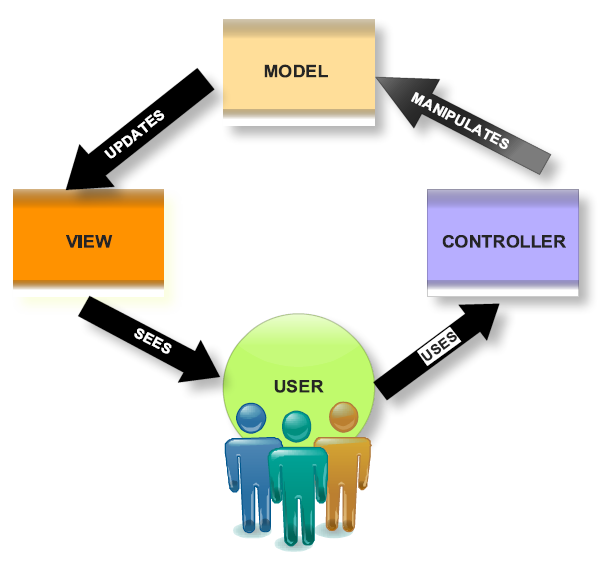
\includegraphics[width=0.5\linewidth]{Gambar/MVC.PNG}
     \caption{Perputaran \textit{Model-View-Controller}}
     \label{fig:label}
 \end{figure}
Gambar \ref{fig:label} menunjukkan pola dan interaksi dengan pengguna dan aplikasi itu sendiri. Ini adalah tata letak aliran tunggal data, bagaimana data itu dilewatkan di antara setiap komponen, dan akhirnya bagaimana hubungan antara setiap komponen bekerja. 


\subsubsection{\textit{Model}}
\label{sec:Model}
\textit{Model} bertujuan untuk memberikan penyimpanan permanen data yang digunakan dalam desain keseluruhan \cite{codeigniter}. Hal tersebut mewajibkan model untuk dapat mengakses data untuk dilihat, atau dikumpulkan dan ditulis, dan merupakan jembatan antara komponen View dan komponen Controller. Salah satu aspek penting dari Model adalah bahwa secara teknis "buta". Dengan ini, \textit{Model} tidak memiliki koneksi atau pengetahuan tentang apa yang terjadi pada data ketika diteruskan ke komponen \textit{View} atau \textit{Controller}. \textit{Model}  tidak memanggil atau mencari tanggapan dari bagian lain dari komponen. Tujuan utamanya adalah untuk mengolah data menjadi penyimpanan permanennya, mencari dan menyiapkan data untuk diteruskan ke bagian lain. 

\textit{Model} tidak dapat dianggap hanya sebagai perangkat database saja, atau pintu gerbang ke sistem lain yang menangani proses data. \textit{Model} mewakili penjaga gerbang ke data itu sendiri, tidak mengajukan pertanyaan tetapi menerima semua permintaan yang datang. Seringkali bagian paling kompleks dari sistem MVC ini, komponen \textit{Model} juga merupakan puncak dari keseluruhan sistem karena tanpanya tidak akan ada koneksi antara \textit{Controller} dan \textit{View} .

\subsubsection{\textit{View}}
\label{sec:View} 
View merupakan informasi yang diminta dari \textit{Model} dan ditampilkan kepada pengguna \cite{codeigniter}. Secara tradisional, dalam aplikasi web menggunakan MVC untuk pengembangan, View adalah bagian dari sistem dimana HTML dihasilkan dan ditampilkan. View juga memicu reaksi dari pengguna yang kemudian berinteraksi dengan \textit{controller}. Contoh dasar dari ini adalah tombol yang dihasilkan oleh \textit{view}, yang di klik oleh pengguna dan memicu tindakan pada \textit{controller}. 

Namun terkadang beberapa orang memiliki konsep yang salah terhadap \textit{View}, terutama oleh pengguna yang mengembangkan web dengan menggunakan pola MVC untuk membangun aplikasi mereka. Sebagai contoh, banyak yang salah mengira bahwa \textit{View} tidak memiliki koneksi apa pun dengan \textit{Model} dan bahwa semua data yang ditampilkan oleh \textit{View} dilewatkan dari \textit{Controller}. Pada kenyataannya, aliran ini mengabaikan teori di balik pola MVC sepenuhnya.Untuk menerapkan arsitektur MVC dengan benar, tidak boleh ada interaksi antara \textit{Model} dengan \textit{View}. Semua logika hanya ditangani oleh \textit{Controller}. Selain itu, deskripsi \textit{View} sebagai file template pun tidak tepat. \textit{View} merupakan sesuatu yang lebih dari sekadar template. Kerangka kerja yang terinspirasi MVC modern telah merusak tampilan hampir ke titik di mana kurangnya  kepedulian apakah kerangka kerja benar-benar mematuhi pola MVC yang benar atau tidak. Penting juga untuk menyebutkan bahwa bagian \textit{View} tidak pernah diberikan data oleh \textit{Controller}. Tidak ada hubungan langsung antara \textit{View} dan \textit{Controller} tanpa \textit{Model} di antara keduanya.  

\subsubsection{\textit{Controller}}
\label{sec:Controller} 
Komponen ketiga dari MVC adalah \textit{Controller}. Tugasnya adalah menangani data yang dikirimkan pengguna serta memperbarui \textit{Model} yang sesuai \cite{codeigniter}. \textit{Controller} dapat disimpulkan sebagai pengumpul informasi, yang kemudian diteruskan ke \textit{Model} untuk diatur penyimpanannya, dan tidak mengandung logika apa pun selain mengumpulkan masukan dari pengguna. \textit{Controller} juga hanya terhubung ke \textit{View} tunggal dan \textit{Model} tunggal, menjadikannya sistem aliran data satu arah, dengan jabat tangan dan tanda tangan di setiap titik pertukaran data. \textit{Controller} hanya diberikan tugas untuk dilakukan saat pengguna sedang berinteraksi dengan \textit{View} dan setiap fungsi \textit{Controller} adalah sebuah pemicu, yang dipicu oleh interaksi antara pengguna dengan \textit{View}. Kesalahan paling umum yang dibuat oleh pengembang adalah menganggap \textit{Controller} sebagai \textit{gateway}, dan akhirnya menetapkan fungsi dan tanggung jawab yang seharusnya dilakukan oleh \textit{View} (ini biasanya merupakan hasil dari pengembang yang sama yang mengacaukan komponen \textit{View} sebagai template). Selain itu, adalah kesalahan umum untuk menetapkan fungsi \textit{Controller} yang memberikan tanggung jawab tunggal untuk mengolah, meneruskan, dan memproses data dari \textit{Model} ke \textit{View}. Meskipun demikian, hubungan pola MVC harus dijaga antara \textit{Model} dan \textit{View}. 

\section{BASH}
\label{sec:BASH}
BASH adalah penerjemah default pada banyak sistem GNU/Linux yang merupakan singkatan dari \textit{Bourne Again SHell}, Bash adalah  shell yang kompatibel yang menggabungkan fitur berguna dari \textit{Korn shell} (ksh) dan \textit{C Shell}(csh)\footnote{\url{https://www.gnu.org/software/bash/}}. BASH menawarkan peningkatan fungsional atas sh untuk pemrograman dan penggunaan interaktif. Selain itu, sebagian besar skrip shell dapat dijalankan oleh Bash tanpa modifikasi. Kelebihan yang dapat diberikan oleh Bash antara lain sebagai berikut
\begin{itemize}
    \item Edit pada \textit{command-line}
    \item Riwayat penulisan perintah yang tidak dibatasi
    \item Kontrol pekerjaan
    \item Fungsi dari shell
    \item array dengan index tidak terbatas
    \item bilangan integer dari hanya 2 bit sampai 64 bit
\end{itemize}

\section{SharIF-Judge}
\label{sec: SharIF-Judge}
Sharif Judge adalah online judge gratis untuk bahasa pemrograman C, C++, Java dan Python \footnote{\url{https://github.com/mjnaderi/Sharif-Judge}}. Perangkat lunak ini diciptakan oleh Mohammad Javad Naderi pada tahun 2014 dan bersifat open source. Antarmuka Sharif Judge ditulis menggunakan bahasa pemrograman PHP (framework CodeIgniter) dan backend menggunakan BASH.
erikut ini merupakan fitur-fitur yang dimiliki oleh Sharif Judge antara lain yaitu:
\begin{itemize}
    \item {\textit{Multiple Role}}\newline
        Pada SharIF-Judge, \textit{User} memiliki 4 jenis \textit{role} yang dibedakan berdasarkan level, dimana level tersebut digunakan untuk memisahkan aksi yang dapat dilakukan setiap \textit{role}. 4 \textit{role} tersebut adalah \textit{Admin}, \textit{Head Instructor}, \textit{Instructor}, dan \textit{Student}. 
        
    \begin{table}[H] %atau h saja untuk "kira kira di sini"
	    \centering 
	    \caption{Tabel \textit{role}}
	    \label{tab:level}
	    \begin{tabular}{|c|c|}
		    \hline
		    \textit{Role} & Level \\
		    \hline
		    \textit{Admin} & 3 \\
		    \hline
		    \textit{Head Instructor} & 2 \\
		    \hline
		    \textit{Instructor} & 1 \\
		    \hline
		    \textit{Student} & 0 \\
		    \hline
	    \end{tabular} 
    \end{table}
    
        Pada Tabel \ref{tab:level} menunjukan level role yang ada pada SharIF-Judge. Setiap \textit{role} tersebut, dapat melakukan aksi yang berbeda-beda yang disesuaikan dengan level role. Untuk melihat aksi apa saja yang dapat dilakukan setiap \textit{role} dapat dilihat pada Tabel \ref{tab:aksi}.
    \begin{table}[H]
	    \centering 
	    \caption{Tabel \textit{Action}}
	    \label{tab:aksi}
	    \begin{tabular}{|c|c|c|c|c|}
		    \hline
		    \textit{Action} & \textit{Admin} & \textit{Head Instructor} & \textit{Instructor} & \textit{Student} \\
		    \hline
		    Mengubah \textit{Setting} & O & X & X & X \\
		    \hline
		    Menambah/Menghapus \textit{User} & O & X & X & X \\
		    \hline
		    Mengubah \textit{role users} & O & X & X & X \\
		    \hline
		    Menambah/Menghapus/Mengubah \textit{Assignment} & O & O & X & X \\
		    \hline
		    Mengunduh \textit{Test} & O & O & X & X \\
		    \hline
		    Menambah/Menghapus/Mengubah Notifikasi & O & O & X & X \\
		    \hline
		    Rejudge & O & O & X & X \\
		    \hline
		    Melihat/Pause/Melanjutkan/Submission Queue & O & O & X & X \\
		    \hline
		    Mendeteksi Kode yang Mirip  & O & O & X & X \\
		    \hline
		    Melihat Semua Kode  & O & O & O & X \\
		    \hline
		    Mengunduh Kode Final  & O & O & O & X \\
		    \hline
		    Memilih \textit{Assignment}   & O & O & O & O \\
		    \hline
		    Submit  & O & O & O & O \\
		    \hline
	    \end{tabular} 
    \end{table}
        Pengguna dapat menambahkan \textit{user} dengan menggunakan fitur \textit{Add User} pada halaman \textit{User}, Pengguna harus mengisi semua informasi yang ada pada text area. Baris dimulai dengan komentar
\#. Setiap baris lainnya mewakili pengguna dengan sintaks berikut:
\hspace{-10mm}

    \begin{verbatim}
USERNAME EMAIL PASSWORD ROLE
        
- Username dapat berisikan huruf kecil atau nomor dan harus terdiri antara 3 
  sampai 20 karakter.
- Password harus terdiri antara 6 sampai 30 karakter.
- Pengguna dapat menggunakan RANDOM[n] untuk menghasilkan password acak yang
  terdiri dari n-digit karakter.
- ROLE harus terdiri dari salah satu yang disebutkan sebagai berikut:‘admin‘,
  ‘head_instructor‘, ‘instructor‘, dan ‘student‘
    \end{verbatim}
    \vspace{-4mm}
    Berikut ini adalah contoh penggunaan sintaks untuk \textit{add user}:
    \begin{verbatim}
# This is a comment!
# This is another comment!
instructor instructor@sharifjudge.ir 123456 head_instructor
instructor2 instructor2@sharifjudge.ir random[7] instructor
student1 st1@sharifjudge.ir random[6] student
student2 st2@sharifjudge.ir random[6] student
student3 st3@sharifjudge.ir random[6] student
student4 st4@sharifjudge.ir random[6] student
student5 st5@sharifjudge.ir random[6] student
student6 st6@sharifjudge.ir random[6] student
student7 st7@sharifjudge.ir random[6] student
    \end{verbatim}
    \vspace{-5mm}
    \item \textit{Sandboxing}\newline
        \textit{Sandboxing} adalah sebuah mekanisme dimana sebuah aplikasi yang dikirimkan oleh pengguna, dapat dijalankan dalam lingkungan virtual yang aman dan menghindari adanya serangan keluar dari Sharif Judge. \\
    \item \textit{Cheat Detection}
    
    \textit{Cheat Detection} berguna sebagai pendeteksi adanya kode yang mirip dan sebagai pendeteksi kecurangan. Untuk pengecekan digunakan MOSS(\textit{Measure Of Software Similarity}) Moss adalah perangkat lunak yang digunakan oleh guru dan penerbit untuk menemukan plagiarisme perangkat lunak. Perangkat lunak ini dikembangkan oleh Stanford, dan telah menjadi alat utama untuk memeriksa plagiarisme kode. MOSS diciptakan untuk menghentikan kelaziman pada siswa untuk menyalin kode dan langsung selesai tanpa adanya pengertian dari siswa terhadap pelajaran tersebut\footnote{\url{https://codequiry.com/moss/measure-of-software-similarity}}. \\
    \item Penilaian berbeda untuk keterlambatan pengumpulan
    
    Hal ini berguna agar jika pelajar ada yang membutuhkan pengertian khusus dan memiliki alasan yang baik, pengajar dapat memberikan pengecualian dan memberikan hukuman ringan.\\
    \item Antrian pengiriman \newline
    Hal ini berguna agar Sharif Judge tidak \textit{down} akibat banyaknya pengiriman.\\
    
    \item Mengunduh nilai dalam bentuk \textit{excel}\newline
    Hal ini berguna agar pengajar tidak mendapatkan kesulitan untuk menyimpan data nilai pelajar.\\
    
    \item Mengunduh kode yang dikumpulkan dalam bentuk zip \newline
    Hal ini berguna agar ketika kode yang harus dikumpulkan ada banyak dan ketika pengajar ingin memeriksa, file tersedia dengan rapih. \\
    
    \item Metode "Output Comparison" dan "Tester Code" untuk memeriksa \textit{output}. \newline
    Hal ini berguna agar pelajar mengetahui apakah pekerjaan yang dikirimkan tersebut sudah benar atau masih kurang tepat. \\
    
    \item Penilaian ulang \newline
    Hal ini berguna agar ketika pengajar melakukan kesalahan penilaian, pengajar dapat melakukan edit. \\
    \item Papan nilai\newline
    Hal ini berguna agar pelajar dapat melihat nilai dari pelajar-pelajar yang lain dan bisa menjadi motivasi bagi pelajar tersebut. \\
    \item Notifikasi \newline
    hal ini berguna agar ketika ada tugas yang harus dikumpulkan, pelajar mengetahuinya dan tidak terlewat.
\end{itemize}

\subsection{Instalasi}
\label{sec:Instalasi}
Untuk dapat menjalankan Sharif Judge, diwajibkan untuk memiliki server Linux dan mengikuti tahapan sebagai berikut\footnote{\url{https://github.com/mjnaderi/Sharif-Judge}\label{github}}:
\begin{itemize}
    \item Menjalankan PHP versi 5.3 atau versi yang lebih baru.
    \item Pengguna dapat menjalankan PHP dari command line  dan pengguna perlu menginstall paket PHP CLI.
    \item Memiliki \textit{Mysql} atau \textit{PostgreSql databse}.
    \item PHP memiliki akses untuk menjalankan perintah \textit{shell} terutama untuk fungsi \textit{shell\_exec}. contohnya seperti \textit{command} di bawah ini: 
    \vspace{-2mm}
    \begin{verbatim}
        echo shell_exec(``php -v'');
    \end{verbatim}
    \vspace{-5mm}
    \item Untuk melakukan proses kompilasi dan menjalankan kode yang dikumpulkan adalah (\textit{gcc, g++, javac, java, python2, python3 commands})
    \item Disarankan untuk melakukan instalasi \textit{Perl} dengan alasan agar memiliki ketepatan waktu, penggunaan \textit{memory} yang terbatas dan memaksimalkan batas ukuran pada \textit{output} kode yang dikirimkan.
\end{itemize}
Jika persyaratan diatas telah selesai dilakukan, dapat melakukan instalasi sebagai berikut: 
\begin{itemize}
    \item Mengunduh versi terakhir dari Sharif Judge dan unpack file yang berhasil diunduh, letakan pada direktori html publik
    \item Untuk mempermudah pindahkan folder \textit{system}  dan \textit{application} keluar dari direktori publik dan masukan \textit{path} lengkap pada file index.php
    \vspace{-2mm}
    \begin{verbatim}
        $system_path = `/home/mohammad/secret/system`;
        $application_folder = `/home/mohammad/secret/application`;
    \end{verbatim}
    \vspace{-5mm}
    \item Membuat sebuah \textit{Mysql} atau \textit{PostgreSql database} untuk Sharif Judge.
    \item Mengatur koneksi database di file application/config/database.php.
    \vspace{-2mm}
    \begin{verbatim}
/* Enter database connection settings here: */
’dbdriver’ => ’postgre’, // database driver (mysqli, postgre)
’hostname’ => ’localhost’, // database host
’username’ => ‘, // database username
’password’ => ‘, // database password
’database’ => ‘, // database name
’dbprefix’ => ’shj_’, // table prefix
/**********************************************/
    \end{verbatim}
    \vspace{-5mm}
    \item Membuat direktori application/cache/Twig agar dapat ditulis oleh PHP
    \item Membuka halaman utama Sharif Judge pada web browser \item \textit{Log in}  menggunakan akun \textit{admin}
    \item Memindahkan folder \textit{tester} dan \textit{assigments} di luar direktori publik lalu simpan \textit{path} lengkap pada halaman \textit{Settings} . Dua folder tersebut harus dapat ditulis oleh PHP. File-file yang diunggah akan disimpan di folder \textit{assigments} sehingga tidak dapat diakses publik.
\end{itemize}

\subsection{\textit{Add Assignment}}
Pengguna dapat menambahkan \textit{assignment} dengan cara mengklik menu \textit{Assignments} lalu klik \textit{add} pada halaman tersebut\footref{github}. Pada Gambar \ref{fig:addAssignment} merupakan halaman \textit{add assignment}.
 \begin{figure}[h!]
     \centering
     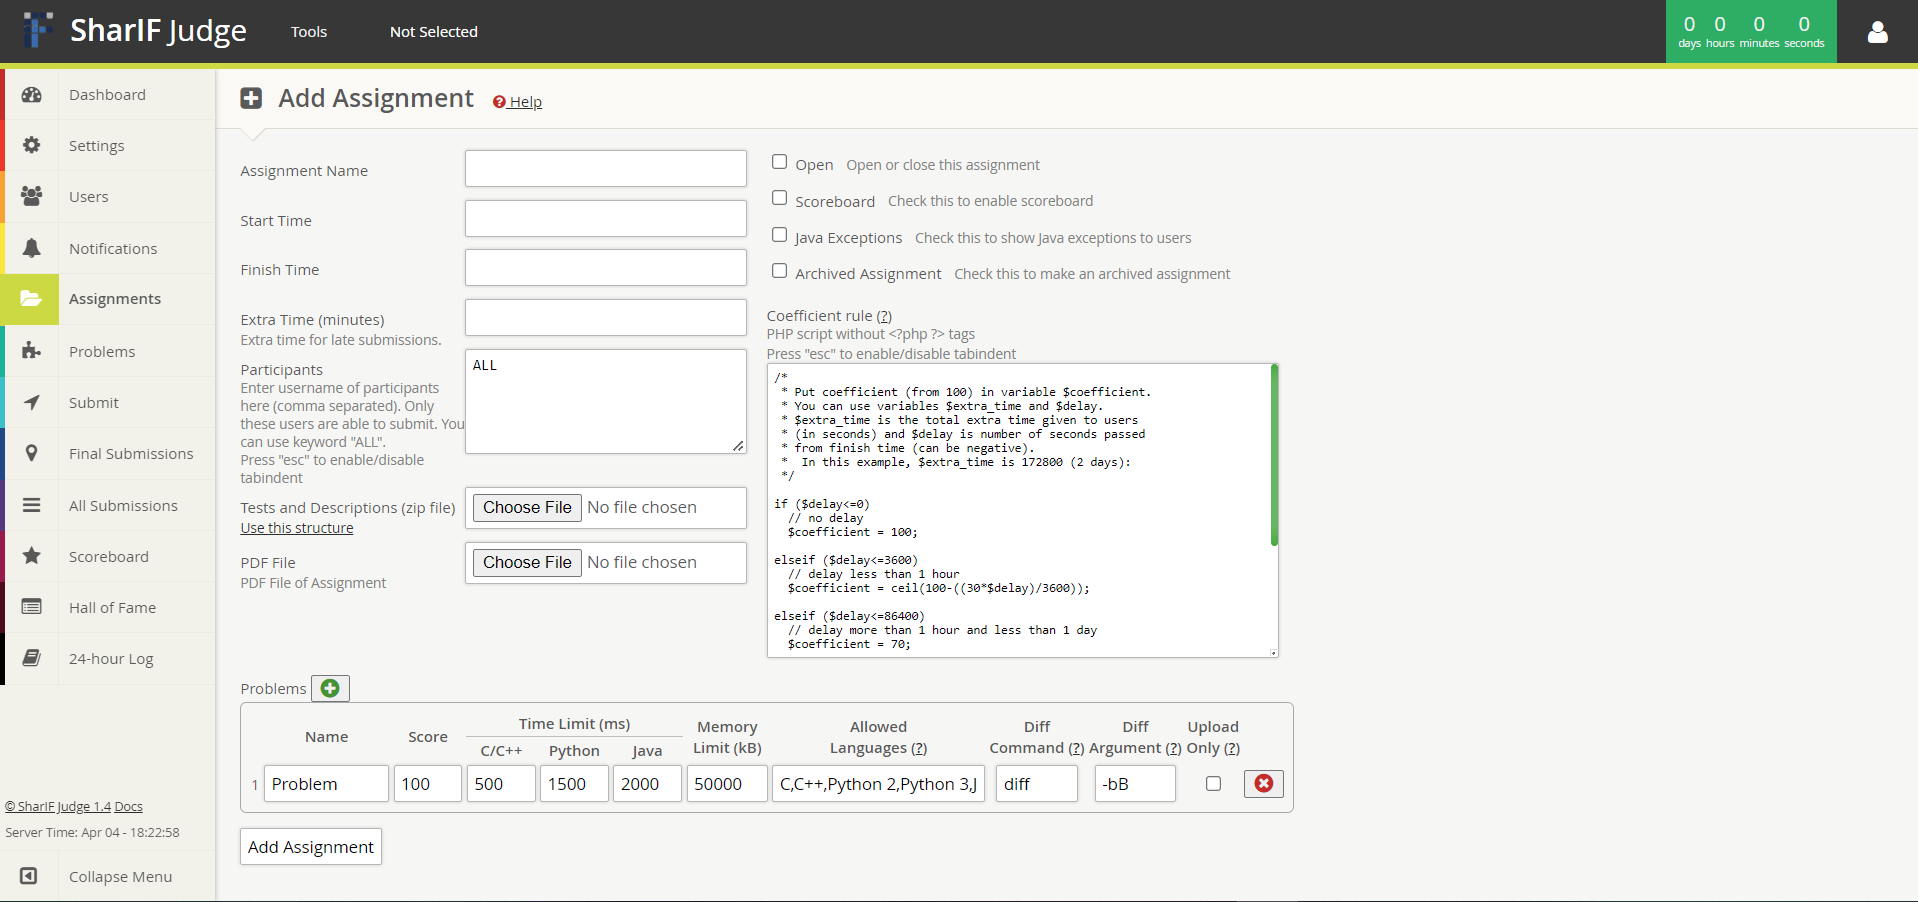
\includegraphics[width=1\linewidth]{Gambar/Add Assignment.PNG}
     \caption{Halaman \textit{Assignment}}
     \label{fig:addAssignment}
 \end{figure}
Berikut ini merupakan pengaturan yang terdapat pada \textit{add assignment}: 
\begin{itemize}
    \item \textit{Assignment Name}\newline
    Memberikan nama pada \textit{assignment} yang akan dibuat \\
    \item \textit{Start Time}\newline
    Menentukan dimulainya waktu dari \textit{assignment} tersebut dan peserta tidak dapat mengumpulkan \textit{assignment} tersebut lebih cepat dari \textit{start time}. Format yang digunakan untuk \textit{start time} adalah \textit{MM/DD/YYYY HH:MM:SS}. Contoh penulisannya adalah 08/31/2013 12:00:00 \\
    \item \textit{Finish Time and Extra Time}\newline
    Peserta tidak dapat melakukan aksi \textit{submit} setelah \textit{Finish time + Extra time}. \textit{Assignment} yang telat akan dikalikan dengan koefisien yang sudah ditentukan. Pengguna harus menulis \textit{script} dalam bahasa PHP untuk menghitung koefisien pada bidang "\textit{Coefficient Rule}". Format yang digunakan dalam pengaturan \textit{finish time} adalah \textit{MM/DD/YYYY HH:MM:SS}. Contoh penulisannya adalah 08/31/2013 23:59:59. "Extra Time" akan terhitung dalam satuan menit. Pengguna juga dapat menggunakan operator aritmatika seperti *, -, +, /. Contoh 120 (2 jam) atau 48*60 (2 hari).\\
    \item \textit{Participants} \newline
    Pengaturan ini berfungsi untuk membatasi peserta yang dapat mengumpulkan assignment. Pengguna dapat menggunakan kata kunci \textit{ALL} pada kolom \textit{Participants} untuk mengijinkan seluruh peserta agar dapat mengumpulkan \textit{assignment}. Untuk membatasi peserta tertentu, pengguna dapat memasukan username peserta pada kolom \textit{Participants}. Setiap username dapat dipisahkan menggunakan tanda koma. Contoh: admin, instructor1, instructor2, student1.\\
    \item \textit{Tests}\newline
    Pengguna dapat mengirim tes kasus dalam \textit{file} zip dengan syarat saat menambahkan tugas, Pengguna harus menyediakan file zip yang berisi kasus uji. File zip ini harus berisi folder untuk setiap masalah (masalah Upload-Only tidak memerlukan folder apa pun). Nama folder harus p1, p2, p3, \ldots Metode yang dapat digunakan untuk memeriksa keluaran setiap masalah adalah dengan metode “Perbandingan \textit{Input/Output}” dan metode “\textit{Tester}”.
    \begin{itemize}
        \item Perbandingan \textit{Input/Output} \newline
        Dalam metode ini, Pengguna harus meletakkan beberapa file \textit{input} dan \textit{output} di folder masalah. SharIF-Judge memberikan setiap file input tes ke kode pengguna dan membandingkan output pengguna dengan output tes. File input harus di folder in dengan nama input1.txt, input2.txt, \ldots dan file output harus di folder out dengan nama output1.txt, output2.txt, \ldots
        \item \textit{Tester}\newline
        Dalam metode ini, Pengguna harus menyediakan beberapa file pengujian input dan file C++ (tester.cpp) dan (opsional) beberapa file pengujian output. SharIF-Judge memberikan file tes input ke kode pengguna dan mendapatkan output pengguna. Kemudian tester.cpp mendapatkan input tes, output tes, dan output pengguna. Jika output pengguna benar, mengembalikan 0, jika tidak mengembalikan 1.
        Pengguna dapat menggunakan template kode ini untuk menulis tester.cpp: 
        \begin{verbatim}
/*
 * tester.cpp
 */
 
#include <iostream>
#include <fstream>
#include <string>
using namespace std;
int main(int argc, char const *argv[])
{
 
	ifstream test_in(argv[1]);  /* This stream reads from test's input file  */
	ifstream test_out(argv[2]); /* This stream reads from test's output file */
	ifstream user_out(argv[3]); /* This stream reads from user's output file */
 
	/* Your code here */
	/* If user's output is correct, return 0, otherwise return 1       */
 
	...
 
}
        \end{verbatim}
        Diberikan contoh dari file tes kasus dengan struktur file sebagai berikut:
        \begin{verbatim}
.
|-- p1
|   |-- in
|   |   |-- input1.txt
|   |   |-- input2.txt
|   |   |-- input3.txt
|   |   |-- input4.txt
|   |   |-- input5.txt
|   |   |-- input6.txt
|   |   |-- input7.txt
|   |   |-- input8.txt
|   |   |-- input9.txt
|   |   |-- input10.txt
|   |-- out
|   |   |-- output1.txt
|   |-- tester.cpp
|-- p2
    |-- in
    |   |-- input1.txt
    |   |-- input2.txt
    |   |-- input3.txt
    |   |-- input4.txt
    |   |-- input5.txt
    |   |-- input6.txt
    |   |-- input7.txt
    |   |-- input8.txt
    |   |-- input9.txt
    |   |-- input10.txt
    |-- out
        |-- output1.txt
        |-- output2.txt
        |-- output3.txt
        |-- output4.txt
        |-- output5.txt
        |-- output6.txt
        |-- output7.txt
        |-- output8.txt
        |-- output9.txt
        |-- output10.txt   
        \end{verbatim}
    \end{itemize}
        \item \textit{Open} \newline
        Pengguna dapat membuka atau menutup \textit{assignment} menggunakan pilihan ini. Jika pengguna menutup \textit{assignment}, \textit{non-student users} masih dapat mengumpulkan \textit{assignment}. \\
        \item \textit{Scoreboard} \newline
        Pengguna dapat mengaktifkan atau mematikan papan nilai dengan menggunakan pilihan ini.
        \item \textit{Java Exceptions} \newline
        Pengguna dapat mengaktifkan dan mematikan java exceptions yang ditunjukan kepada \textit{role students}. Perubahan pada pilihan ini tidak berdampak pada kode yang sebelumnya sudah dinilai. Nama \textit{exception} akan muncul ketika pada file pathtester/java\_exceptions\_list berisikan nama \textit{exception} tersebut. Berikut hasil exception yang ditunjukan jika pengguna mengaktifkan pengaturan \textit{Java Exceptions}:
        \begin{verbatim}
Test 1
ACCEPT
Test 2
Runtime Error (java.lang.ArrayIndexOutOfBoundsException)
Test 3
Runtime Error (java.lang.ArrayIndexOutOfBoundsException)
Test 4
ACCEPT
Test 5
ACCEPT
Test 6
ACCEPT
Test 7
ACCEPT
Test 8
Runtime Error (java.lang.ArrayIndexOutOfBoundsException)
Test 9
Runtime Error (java.lang.StackOverflowError)
Test 10
Runtime Error (java.lang.ArrayIndexOutOfBoundsException)
        \end{verbatim}
        \item \textit{Coefficient Rule} \newline
        Pengguna dapat menulis skrip PHP di sini yang menghitung koefisien dikalikan dengan skor. Skrip pengguna harus memasukkan koefisien (dari 100) ke dalam variabel \$koefisien. Pengguna dapat menggunakan variabel \$extra\_time dan \$delay. \$extra\_time adalah total waktu tambahan yang diberikan kepada pengguna dalam detik (waktu tambahan yang Anda masukkan di bidang Extra Time) dan \$delay adalah jumlah detik yang berlalu dari waktu selesai (bisa negatif). Skrip PHP ini tidak boleh mengandung tag <?php , <? , ?>. Dalam contoh ini, \$extra\_time adalah 172800 (2 hari): 
        \begin{verbatim}
if ($delay<=0)
  // no delay
  $coefficient = 100;

elseif ($delay<=3600)
  // delay less than 1 hour
  $coefficient = ceil(100-((30*$delay)/3600));

elseif ($delay<=86400)
  // delay more than 1 hour and less than 1 day
  $coefficient = 70;

elseif (($delay-86400)<=3600)
  // delay less than 1 hour in second day
  $coefficient = ceil(70-((20*($delay-86400))/3600));

elseif (($delay-86400)<=86400)
  // delay more than 1 hour in second day
  $coefficient = 50;

elseif ($delay > $extra_time)
  // too late
  $coefficient = 0;
        \end{verbatim}
    \item \textit{Time Limit} \newline
    Pengguna dapat mengatur batas waktu dalam menjalankan kode dalam satuan milisekon. Program yang ditulis menggunakan Python dan Java biasanya lebih lambat dari C/C++. Oleh karena itu Python dan Java membutuhkan waktu yang lebih lama. \\
    \item \textit{Memory Limit} \newline
    Pengguna dapat mengatur batas memori dalam satuan kilobyte, namun penggunaan \textit{Memory Limit} tidak terlalu akurat.\\
    \item \textit{Allowed Languages} \newline
    Melakukan pengaturan bahasa untuk setiap kasus yang dipisahkan menggunakan koma. Bahasa yang tersedia seperti C, C++, Java, Python 2, Python 3, zip, PDF. Pengguna dapat menggunakan zip atau PDF jika mengaktifkan pilihan Upload Only. Contoh: C, C++ , zip atau Python 2,Python 3 atau Java ,C. \\
    \item \textit{Diff Command} \newline
    \textit{Command} ini digunakan untuk membandingkan keluaran dengan keluaran yang benar. Secara default SharIF-Judge menggunakan \textit{diff}, namun pengguna dapat mengubah \textit{command} pada bagian ini. \\
    \item \textit{Diff Arguments} \newline
    Pengguna dapat mengatur argumen dari \textit{Diff Command} disini. Untuk melihat daftar lengkap \textit{diff argumen}, pengguna dapat melihat \textit{man diff}. SharIF-Judge menambahkan dua pilihan baru yaitu \textit{ignore} dan \textit{identical}. \textit{Ignore} akan menghiraukan semua baris baru dan spasi. \textit{Identical} tidak akan menghiraukan apapun namun keluaran dari file yang dikumpulkan harus identik dengan keluaran test case agar dapat diterima. \\
    \item \textit{Upload Only} \newline
    Jika pengguna mengatur problem sebagai \textit{Upload-Only}, maka SharIF-Judge tidak akan menilai \textit{assignment} pada kasus tersebut. Pengguna dapat menggunakan zip dan PDF pada \textit{allowed languages} jika mengaktifkan pilihan ini.
\end{itemize}
\newpage
Perhatikan bawa berbeda dengan penempatan judul gambar gambar, keterangan tabel harus diletakkan di atas tabel!!
Lihat Tabel~\ref{tab:contoh1} berikut ini:

\begin{table}[H] %atau h saja untuk "kira kira di sini"
	\centering 
	\caption{Tabel contoh}
	\label{tab:contoh1}
	\begin{tabular}{cccc}
		\toprule
		& $v_{start}$ & $\mathcal{S}_{1}$ & $v_{end}$\\

		\midrule
		$\tau_{1}$ & 1 & 12& 20\\
		$\tau_{2}$ & 1 &  & 20\\
		$\tau_{3}$ & 1 & 9 & 20\\
		$\tau_{4}$ & 1 &  & 20\\

		\bottomrule
		
	\end{tabular} 
\end{table}
Tabel~\ref{tab:cthwarna1} dan Tabel~\ref{tab:cthwarna2} berikut ini adalah tabel dengan sel yang berwarna dan ada dua tabel yang bersebelahan. 
\begin{table}[H]
	\begin{minipage}[c]{0.49\linewidth}
		\centering
		\caption{Tabel bewarna(1)}
		\label{tab:cthwarna1}
		\begin{tabular}{ccccc}
			\toprule
			 & $v_{start}$ & $\mathcal{S}_{2}$ & $\mathcal{S}_{1}$ & $v_{end}$\\
			
			\midrule
			$\tau_{1}$ & 1 & 5 \cellcolor{green}& 12& 20\\
			$\tau_{2}$ & 1 & 8 \cellcolor{green}& & 20\\
			$\tau_{3}$ & 1 & 2/8/17 \cellcolor{green}& 9 & 20\\
			$\tau_{4}$ & 1 & \cellcolor{red}& & 20\\
			
			\bottomrule

		\end{tabular}
	\end{minipage}
	\begin{minipage}[c]{0.49\linewidth}
		
		\centering 
		\caption{Tabel bewarna(2)}
		\label{tab:cthwarna2}
		\begin{tabular}{ccccc}
			\toprule
			 & $v_{start}$ & $\mathcal{S}_{1}$ & $\mathcal{S}_{2}$ & $v_{end}$\\
			
			\midrule
			$\tau_{1}$ & 1 & 12& 5 \cellcolor{red} &20\\
			$\tau_{2}$ & 1 &  &  8 \cellcolor{green} &20\\
			$\tau_{3}$ & 1 & 9 & 2/8/17 \cellcolor{green} &20\\
			$\tau_{4}$ & 1 &   & \cellcolor{red} &20\\
			
			\bottomrule
		
		\end{tabular}
	\end{minipage}
\end{table}

 
\subsection{Kutipan}
\label{subs:kutipan} 
Berikut contoh kutipan dari berbagai sumber, untuk keterangan lebih lengkap, silahkan membaca file referensi.bib yang disediakan juga di template ini.
Contoh kutipan:
\begin{itemize}
	\item Buku:~\cite{berg:08:compgeom} 
	\item Bab dalam buku:~\cite{kreveld:04:GIS}
	\item Artikel dari Jurnal:~\cite{buchin:13:median}
	\item Artikel dari prosiding seminar/konferensi:~\cite{kreveld:11:median}
	\item Skripsi/Thesis/Disertasi:~\cite{lionov:02:animasi}~\cite{wiratma:10:following}~\cite{wiratma:22:later}
	\item Technical/Scientific Report:~\cite{kreveld:07:watertight}
	\item RFC (Request For Comments):~\cite{RFC1654}
	\item Technical Documentation/Technical Manual:~\cite{Z.500}~\cite{unicode:16:stdv9}~\cite{google:16:and7}
	\item Paten:~\cite{webb:12:comm}
	\item Tidak dipublikasikan:~\cite{wiratma:09:median}~\cite{lionov:11:cpoly}
	\item Laman web:~\cite{erickson:03:cgmodel}  
	\item Lain-lain:~\cite{agung:12:tango}
\end{itemize}    
  
\subsection{Gambar}

Pada hampir semua editor, penempatan gambar di dalam dokumen \LaTeX{} tidak dapat dilakukan melalui proses {\it drag and drop}.
Perhatikan contoh pada file bab2.tex untuk melihat bagaimana cara menempatkan gambar.
Beberapa hal yang harus diperhatikan pada saat menempatkan gambar:
\begin{itemize}
	\item Setiap gambar {\bf harus} diacu di dalam teks (gunakan {\it field} {\sc label})
	\item {\it Field} {\sc caption} digunakan untuk teks pengantar pada gambar. Terdapat dua bagian yaitu yang ada di antara tanda $[$ dan $]$ dan yang ada di antara tanda $\{$ dan $\}$. Yang pertama akan muncul di Daftar Gambar, sedangkan yang kedua akan muncul di teks pengantar gambar. Untuk skripsi ini, samakan isi keduanya.
	\item Jenis file yang dapat digunakan sebagai gambar cukup banyak, tetapi yang paling populer adalah tipe {\sc png} (lihat Gambar~\ref{fig:ularpng}), tipe {\sc jpg} (Gambar~\ref{fig:ularjpg}) dan tipe {\sc pdf} (Gambar~\ref{fig:ularpdf})
	\item Besarnya gambar dapat diatur dengan {\it field} {\sc scale}.
	\item Penempatan gambar diatur menggunakan {\it placement specifier} (di antara tanda  $[$ dan $]$ setelah deklarasi gambar.
	Yang umum digunakan adalah {\bf H} untuk menempatkan gambar {\bf sesuai} penempatannya di file .tex atau  {\bf h} yang berarti "kira-kira" di sini. \\
	Jika tidak menggunakan {\it placement specifier}, \LaTeX{} akan menempatkan gambar secara otomatis untuk menghindari bagian kosong pada dokumen anda.
	Walaupun cara ini sangat mudah, hindarkan terjadinya penempatan dua gambar secara berurutan. 	
	\begin{itemize}
		\item Gambar~\ref{fig:ularpng} ditempatkan di bagian atas halaman, walaupun penempatannya dilakukan setelah penulisan 3 paragraf setelah penjelasan ini.
		\item Gambar~\ref{fig:ularjpg} dengan skala 0.5 ditempatkan di antara dua buah paragraf. Perhatikan penulisannya di dalam file bab2.tex!
		\item Gambar~\ref{fig:ularpdf} ditempatkan menggunakan {\it specifier} {\bf h}.
	\end{itemize}
\end{itemize}
 
\dtext{17-18}
\begin{figure} 
	\centering  
	\includegraphics[scale=1]{ular-png}  
	\caption[Gambar {\it Serpentes} dalam format png]{Gambar {\it Serpentes} dalam format png} 
	\label{fig:ularpng} 
\end{figure} 

\dtext{19-20}
\begin{figure}[H]
	\centering  
	\includegraphics[scale=0.5]{ular-jpg}  
	\caption[Ular kecil]{Ular kecil} 
	\label{fig:ularjpg} 
\end{figure} 
\dtext{21-22}

\begin{figure}[ht] 
	\centering  
	\includegraphics[scale=1]{ular-pdf}  
	\caption[ {\it Serpentes} betina]{ {\it Serpentes} jantan} 
	\label{fig:ularpdf} 
\end{figure} 
 
\subsection{Kode Program}

Kode program dalam bahasa tertentu seringkali harus ditulis di dalam bab, bukan hanya dilampirkan di bagian Lampiran. 
Kode~\ref{kode:aneh} menampilkan penggunaan karakter-karakter yang umum digunakan dalam sebuah program yang ditulis dengan bahasa C.


\begin{lstlisting}[language=Java, caption=Kode untuk menampilkan karakter-karakter aneh, label=kode:aneh]
// This does not make algorithmic sense, 
// but it shows off significant programming characters.

#include<stdio.h>

void myFunction( int input, float* output ) {
	switch ( array[i] ) {
		case 1: // This is silly code
			if ( a >= 0 || b <= 3 && c != x )
				*output += 0.005 + 20050;
			char = 'g';
			b = 2^n + ~right_size - leftSize * MAX_SIZE;
			c = (--aaa + &daa) / (bbb++ - ccc % 2 );
			strcpy(a,"hello $@?"); 
	}
	count = ~mask | 0x00FF00AA;
}

// Fonts for Displaying Program Code in LATEX
// Adrian P. Robson, nepsweb.co.uk
// 8 October 2012
// http://nepsweb.co.uk/docs/progfonts.pdf

\end{lstlisting}

\subsection{Notasi}

Simbol-simbol (matematika) yang sering digunakan sepanjang penulisan skripsi, dapat dimasukkan ke dalam ``Daftar Notasi''. Daftar ini ada di halaman depan sebelum Bab~\ref{chap:intro}.
Cara memasukkan sebuah simbol ke dalam Daftar Notasi adalah menggunakan perintah \verb|\nomenclature|. Contoh:
\begin{center}
    \verb|\nomenclature[]{$A$}{luas kandang ular}|    
\end{center}
\nomenclature[]{$A$}{luas kandang ular}
\nomenclature[]{$n$}{banyaknya ular}
\nomenclature[]{$k$}{jumlah kepala per seekor ular\nomrefpage}
Argumen opsional digunakan untuk mengurutkan notasi. Silahkan lihat sendiri dokumentasi package \verb|nomencl|

